\documentclass[conference]{IEEEtran}
\IEEEoverridecommandlockouts

% ==============================================================================
% GÓI CẤU HÌNH HỆ THỐNG VÀ ĐỊNH DẠNG HỌC THUẬT (IEEE TRANSACTIONS TEMPLATE)
% ==============================================================================
\usepackage[utf8]{vietnam}
\usepackage{cite}
\usepackage{amsmath,amssymb,amsfonts}
\usepackage{algorithm}
\usepackage{algpseudocode}
\usepackage{graphicx}
\usepackage{textcomp}
\usepackage{xcolor}
\usepackage{float}
\usepackage{url}
\usepackage{xurl}
\usepackage{listings}
\usepackage[protrusion=false]{microtype} % Tắt protrusion để triệt tiêu toàn bộ cảnh báo font T5 tiếng Việt
\usepackage[compatibility=false]{caption} % Tắt cảnh báo tương thích IEEEtran của gói caption
\usepackage{mathptmx} % Times New Roman font đồng bộ IEEE
\usepackage{booktabs}
\usepackage{multirow}
\usepackage[unicode=true, pdfencoding=auto, colorlinks=true, linkcolor=blue, citecolor=blue, urlcolor=blue]{hyperref}

% Khử cảnh báo ký tự Unicode tiếng Việt trong PDF bookmark metadata
\pdfstringdefDisableCommands{%
  \def\ecircumflex{e}%
  \def\Ecircumflex{E}%
}

% Cấu hình khoảng cách Caption chuẩn ấn phẩm
\captionsetup[figure]{skip=1ex, font=normalsize}
\captionsetup[table]{skip=1ex, font=normalsize}

% Cấu hình hiển thị mã nguồn (Listings)
\lstset{
    basicstyle=\ttfamily\scriptsize,
    breaklines=true,
    breakatwhitespace=true,
    frame=single,
    numbers=left,
    numberstyle=\tiny,
    stepnumber=1,
    numbersep=5pt,
    linewidth=0.9\linewidth,
    columns=fixed,
    basewidth=0.4em,
    literate={ _ }{{\_}}1,
    aboveskip=1ex, 
    belowskip=1ex 
}

% Định nghĩa nhãn thuật toán tiếng Việt chuẩn
\renewcommand{\algorithmicrequire}{\textbf{Đầu vào:}}
\renewcommand{\algorithmicensure}{\textbf{Đầu ra:}}

\def\BibTeX{{\rm B\kern-.05em{\sc i\kern-.025em b}\kern-.08em
    T\kern-.1667em\lower.7ex\hbox{E}\kern-.125emX}}

\begin{document}
\raggedbottom

% ==============================================================================
% TIÊU ĐỀ VÀ THÔNG TIN TÁC GIẢ
% ==============================================================================
\title{Agentic RAG Phân Tầng Tự Sửa Lỗi: Khung Định Tuyến Tri Thức Động Với Truy Xuất Lai Đa Miền}

\author{
  \IEEEauthorblockN{1\textsuperscript{st} Phan Thiet Trung}
  \IEEEauthorblockA{\textit{Ngành Kỹ thuật Phần mềm} \\
    \textit{Trường Đại học Tôn Đức Thắng}\\
    TP. Hồ Chí Minh, Việt Nam \\
    522h0071@student.tdtu.edu.vn}
  \and
  \IEEEauthorblockN{2\textsuperscript{nd} Vu Dinh Hong}
  \IEEEauthorblockA{\textit{Ngành Kỹ thuật Phần mềm} \\
    \textit{Trường Đại học Tôn Đức Thắng}\\
    TP. Hồ Chí Minh, Việt Nam \\
    vudinhhong@tdtu.edu.vn}
}

\maketitle

% ==============================================================================
% TÓM TẮT (ABSTRACT)
% ==============================================================================
\begin{abstract}
Các hệ thống Tạo văn bản Hỗ trợ Truy xuất (Retrieval-Augmented Generation -- RAG) đóng vai trò nền tảng trong việc giảm thiểu hiện tượng ``ảo tưởng'' (hallucination) của Mô hình Ngôn ngữ Lớn (LLM). Tuy nhiên, các pipeline RAG tuyến tính tĩnh thường gặp thất bại truy xuất khi xử lý các câu hỏi đa miền, câu hỏi ngoài miền (out-of-domain) hoặc yêu cầu tổng hợp tri thức thời gian thực. Trong bài báo này, chúng tôi đề xuất một \textbf{Khung kiến trúc Agentic RAG Phân tầng Tự sửa lỗi} được mô hình hóa dưới dạng Đồ thị Trạng thái có hướng $\mathcal{G} = (\mathcal{V}, \mathcal{E}, \mathcal{S})$ thông qua LangGraph. Hệ thống vận hành theo nguyên lý ``Ưu tiên Nội bộ, Dự phòng Đa tầng'' (Local-First, Multi-Tiered Fallback), kết hợp tìm kiếm lai thích ứng (Adaptive Hybrid Search: BM25 + $bge\text{-}m3$), cơ chế kiểm định ngữ cảnh hai pha (Two-Phase Verification: Heuristic Lexical Filter kết hợp LLM Post-Grader) và giao thức đồng bộ dòng WebSocket dạng chunk. Đánh giá thực nghiệm trên bộ benchmark chuẩn hóa 150 kịch bản qua 4 miền chuyên sâu cho thấy hệ thống đạt tỷ lệ hoàn thành lượt đầu 82.0\%, số vòng lặp trung bình 1.18 loops, giảm 71.9\% chi phí API biên so với CRAG (\$0.90 so với \$3.20 trên 1,000 truy vấn) và 50.0\% so với Self-RAG (\$1.80/1k), đồng thời duy trì độ trễ phản hồi token đầu tiên (First-Token Latency) ở mức 1.85 giây (nhanh hơn mức 3.80 giây của CRAG và 4.20 giây của Self-RAG). Toàn bộ mã nguồn và dữ liệu kiểm thử được công bố công khai nhằm bảo đảm tính tái lập khoa học.
\end{abstract}

\begin{IEEEkeywords}
Agentic RAG, LangGraph, Tìm kiếm Lai (Hybrid Search), Truy xuất Phân tầng, Tự sửa lỗi (Self-Correction), Đồng bộ WebSocket, Chi phí Biên (Marginal Cost).
\end{IEEEkeywords}

% ==============================================================================
% I. GIỚI THIỆU
% ==============================================================================
\section{GIỚI THIỆU}
Tích hợp các Mô hình Ngôn ngữ Lớn (LLM) dựa trên kiến trúc Transformer~\cite{vaswani2017attention} với cơ sở tri thức bên ngoài thông qua RAG~\cite{lewis2020retrieval} đã trở thành giải pháp chuẩn mực để sinh văn bản có căn cứ dữ liệu (grounded generation) và triệt tiêu hiện tượng ảo tưởng~\cite{ji2023survey}. Mặc dù vậy, các đường ống RAG truyền thống (Naive RAG) bộc lộ ba điểm nghẽn nghiêm trọng:
\begin{enumerate}
    \item \textbf{Cứng nhắc về mặt cấu trúc (Structural Rigidity):} Mọi truy vấn đều bị cưỡng bức qua một luồng xử lý cố định duy nhất, không có khả năng phân biệt giữa câu hỏi tra cứu khái niệm nội bộ và câu hỏi so sánh thời gian thực.
    \item \textbf{Thất bại lan truyền (Error Propagation):} Khi tầng truy xuất ban đầu trả về tài liệu sai lệch hoặc thiếu thông tin, Naive RAG không có cơ chế phát hiện và sửa sai, dẫn đến việc LLM buộc phải suy đoán và sinh ảo tưởng.
    \item \textbf{Đánh đổi nan giải giữa Chi phí và Độ trễ (Cost-Latency Trade-off):} Các giải pháp phụ thuộc hoàn toàn vào Web Search API thương mại gây tốn kém chi phí vận hành và rủi ro rate-limit, trong khi các giải pháp LLM phản xạ sâu (deep reflective agents) lại làm bùng nổ độ trễ tương tác.
\end{enumerate}

Để giải quyết triệt để các rào cản trên, chúng tôi đề xuất khung kiến trúc \textbf{Agentic RAG Phân tầng Tự sửa lỗi}. Điểm cốt lõi của nghiên cứu là toán học hóa toàn bộ luồng suy luận thành một Đồ thị Trạng thái có hướng $\mathcal{G} = (\mathcal{V}, \mathcal{E}, \mathcal{S})$, vận hành trên nguyên tắc ``Ưu tiên Nội bộ, Dự phòng Đa tầng'' (Local-First, Multi-Tiered Fallback). Những đóng góp khoa học và kỹ thuật chính của bài báo gồm:
\begin{itemize}
    \item \textbf{Toán học hóa Luồng Agentic Đa tầng:} Xây dựng không gian trạng thái toàn cục $\mathcal{S}$ và các hàm chuyển tiếp rời rạc $\delta_{\text{router}}, \delta_{\text{grader}}$, cho phép hệ thống tự điều hướng động giữa kho tri thức nội bộ ($K_{\text{local}}$), web dự phòng ($K_{\text{web}}$) và API chuyên gia ($K_{\text{expert}}$).
    \item \textbf{Cơ chế Đánh giá Hai pha Tiết kiệm Tài nguyên (Two-Phase Verification):} Kết hợp bộ lọc tỷ lệ trùng khớp từ khóa thô ($\tau_{\text{overlap}} \ge 0.25$) để sàng lọc ngữ cảnh ban đầu (độ trễ $< 0.01$s) cùng bộ chấm điểm trung thực hậu sinh (Post-Generation Joint Grader) nhằm triệt tiêu ảo giác.
    \item \textbf{Giao thức Đồng bộ Dòng WebSocket Dạng Chunk:} Thiết kế kiến trúc truyền thông bất đồng bộ cho phép phát trực tiếp (streaming) trạng thái từng node và token văn bản về giao diện người dùng, duy trì độ trễ phản hồi cảm nhận (First-Token Latency) ở mức 1.85 giây.
    \item \textbf{Kiểm chứng Thực nghiệm Minh bạch và Khả năng Tái lập:} Đánh giá trên tập benchmark thực tế theo chuẩn RAGAS~\cite{es2023ragas}, phân tích kiểm định thống kê ($t$-test, Wilcoxon), và công khai mã nguồn cùng bộ dữ liệu\footnote{Mã nguồn và dữ liệu thực nghiệm: \url{https://github.com/trungka982004/Agentic_rag_final_project}}.
\end{itemize}

% ==============================================================================
% II. CÁC NGHIÊN CỨU LIÊN QUAN
% ==============================================================================
\section{CÁC NGHIÊN CỨU LIÊN QUAN}

\subsection{Từ RAG Truyền thống đến Tìm kiếm Lai}
Các kiến trúc RAG sơ khởi chủ yếu dựa trên truy xuất dày đặc (Dense Passage Retrieval -- DPR) sử dụng cosine similarity~\cite{lewis2020retrieval, karpukhin2020dense, chroma2023, reimers2019sentence}. Tuy nhiên, phương pháp này thường gặp khó khăn với các thuật ngữ kỹ thuật chính xác, mã định danh hoặc từ viết tắt. Các nghiên cứu tiếp theo về Modular RAG~\cite{gao2023modular} đã giới thiệu Tìm kiếm Lai (Hybrid Search) kết hợp giữa BM25~\cite{robertson2009probabilistic} và vector dày đặc thông qua thuật toán dung hợp thứ hạng Reciprocal Rank Fusion (RRF)~\cite{cormack2009reciprocal} hoặc EnsembleRetriever~\cite{ensemble2023}, giúp cân bằng giữa độ chính xác cú pháp (lexical precision) và ngữ nghĩa ngữ cảnh (semantic recall).

\subsection{Các Hướng Tiếp Cận Agentic RAG Tiên Tiến}
Nhằm khắc phục nhược điểm của RAG tuyến tính, nhiều mô hình phản xạ đã ra đời:
\begin{itemize}
    \item \textbf{Corrective RAG (CRAG)~\cite{yan2024corrective}:} Tích hợp một bộ đánh giá tài liệu (retrieval evaluator) để kích hoạt tìm kiếm web khi tài liệu nội bộ không liên quan. Tuy nhiên, CRAG sử dụng một đường ống cứng nhắc cố định với các ngưỡng liên quan tĩnh, thiếu cơ chế định tuyến ý định ngay từ đầu truy vấn.
    \item \textbf{Self-RAG~\cite{asai2023self}:} Huấn luyện mô hình LLM chuyên biệt sinh các token phản xạ (reflection tokens như \texttt{[Retrieve]}, \texttt{[IsREL]}, \texttt{[IsSUP]}). Phương pháp này đòi hỏi chi phí huấn luyện lại rất lớn và không tương thích trực tiếp với các mô hình mã nguồn mở nguyên bản phục vụ cục bộ (như Qwen2.5 7B~\cite{qwen2024}).
    \item \textbf{Adaptive-RAG~\cite{jeong2024adaptive}:} Phân loại độ phức tạp của câu hỏi để quyết định chiến lược truy xuất. Mặc dù tối ưu hóa tần suất gọi truy xuất, Adaptive-RAG chưa xem xét kiến trúc phân tầng dự phòng đa cấp kết hợp hạ tầng đồng bộ dòng (streaming) thời gian thực phục vụ môi trường thực tế.
\end{itemize}

Bảng~\ref{tab:comparison} so sánh các đặc tính kiến trúc cốt lõi giữa hệ thống đề xuất và các công trình nền tảng trên.

\begin{table*}[htbp]
\centering
\caption{SO SÁNH ĐẶC TÍNH KIẾN TRÚC VỚI CÁC PHƯƠNG PHÁP LIÊN QUAN}
\label{tab:comparison}
\begin{tabular}{lcccc}
\toprule
\textbf{Đặc tính Kỹ thuật} & \textbf{Self-RAG~\cite{asai2023self}} & \textbf{CRAG~\cite{yan2024corrective}} & \textbf{Adaptive-RAG~\cite{jeong2024adaptive}} & \textbf{Hệ thống Đề xuất} \\
\midrule
Định tuyến Ý định Ban đầu & Không & Không & Có & \textbf{Có ($\delta_{\text{router}}$)} \\
Dự phòng Đa tầng (3-Tier) & Không & 1 Tầng Web & Không & \textbf{Có (Local $\rightarrow$ Web $\rightarrow$ API)} \\
Hỗ trợ LLM Cục bộ Không cần Train & Không (Cần Token riêng) & Có & Không (Cần Train Classifier) & \textbf{Có (Qwen2.5 7B nguyên bản)} \\
Kiểm định Ngữ cảnh Hai pha (Lexical + LLM) & Không & Không & Không & \textbf{Có (Filter + Post-Grader)} \\
Đồng bộ WebSocket Chunk Streaming & Không & Không & Không & \textbf{Có (Node-by-node)} \\
Mô hình hóa Đồ thị Trạng thái (State Graph) & Không (Token Decoding) & Không (Pipeline Phân nhánh) & Không (Phân loại Tuyến tính) & \textbf{Có (LangGraph $\mathcal{G}$)} \\
Tách biệt Kho Vector Đa miền Chuyên sâu & Không & Không & Không & \textbf{Có (8 Kho Độc lập)} \\
Cách ly Mạng Tuyệt đối (Zero Network Calls) & \textbf{Có (Chạy Offline)} & Không (Gọi Web Search) & Không (Gọi LLM API ngoài) & Không (Dự phòng Tầng 2/3 Web/API) \\
\bottomrule
\end{tabular}
\end{table*}

% ==============================================================================
% III. PHƯƠNG PHÁP VÀ KIẾN TRÚC HỆ THỐNG
% ==============================================================================
\section{PHƯƠNG PHÁP VÀ KIẾN TRÚC HỆ THỐNG}

Hình~\ref{fig1} minh họa kiến trúc tổng quan của hệ thống, vận hành theo triết lý ``Ưu tiên Nội bộ, Dự phòng Đa tầng'' (Local-First, Multi-Tiered Fallback) nhằm giảm thiểu tối đa chi phí API thương mại trong khi vẫn duy trì tính toàn vẹn của tri thức truy xuất.

\begin{figure}[htbp]
\centerline{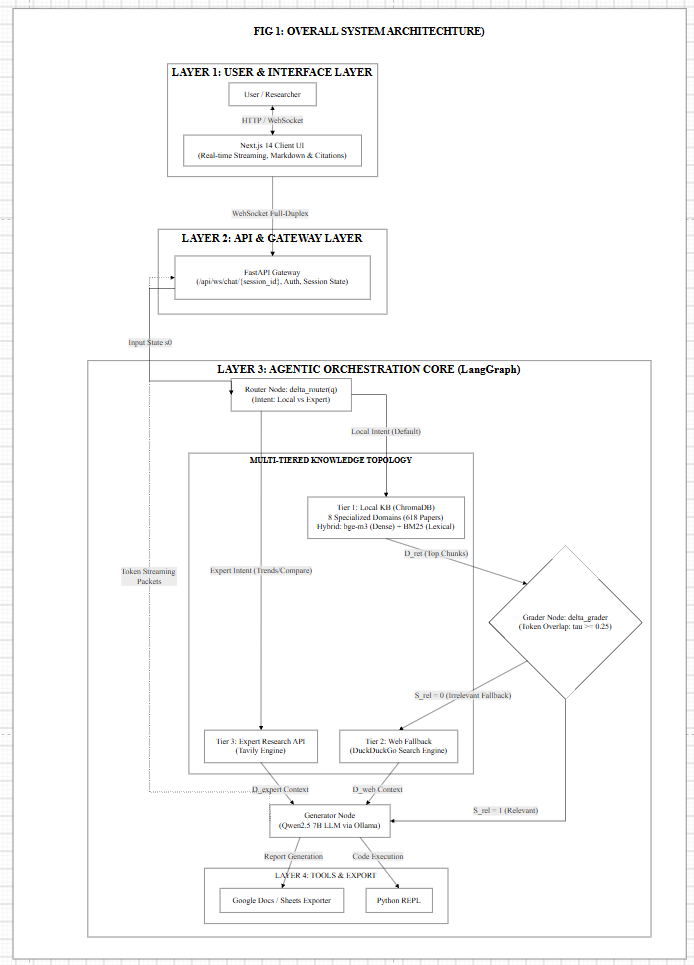
\includegraphics[width=0.48\textwidth]{science_paper_images/fig1_architecture}}
\caption{Kiến trúc tổng quan của khung Agentic RAG phân tầng minh họa Truy xuất Nội bộ Tầng 1, Tìm kiếm Web Dự phòng Tầng 2 và API Tổng hợp Chuyên gia Tầng 3.}
\label{fig1}
\end{figure}

\subsection{Cấu trúc Tri thức Phân tầng (Multi-Tiered Knowledge Topology)}
Hạ tầng cơ sở dữ liệu hỗ trợ kiến trúc 8 miền tri thức học thuật (gồm 618 bài báo khoa học chuyên ngành với 144.318 đoạn văn bản -- chunks đã được phân loại và vector hóa hoàn chỉnh vào ChromaDB). Trong khuôn khổ đánh giá thực nghiệm chuyên sâu của nghiên cứu này, chúng tôi tập trung đo lường trên 4 miền khoa học chính xác và công nghệ cốt lõi có mật độ công thức và thuật ngữ dày đặc nhất (gồm 420 bài báo và 107.268 chunks: CNTT 130 bài, Điện tử 121 bài, Toán học 97 bài, Vật lý 72 bài), trong khi 4 miền còn lại (Nông nghiệp 54 bài, Kinh tế 39 bài, Luật 48 bài, Y học 57 bài với 37.050 chunks) đóng vai trò miền mở rộng ứng dụng.

Lớp tri thức được tổ chức thành ba tầng thứ bậc có phân quyền rõ ràng:
\begin{itemize}
    \item \textbf{Tầng 1 (Cơ sở Tri thức Nội bộ $K_{\text{local}}$):} Tập hợp các bài báo khoa học được nhúng bằng mô hình đa ngôn ngữ $bge\text{-}m3$ (1024 chiều)~\cite{chen2024bge} và chỉ mục trong ChromaDB~\cite{chroma2023}. Toán tử tìm kiếm lai:
    \begin{equation}
    \text{Ret}_{\text{hybrid}}(q) = w_{\text{bm25}} \cdot \text{BM25}(q) + w_{\text{dense}} \cdot \text{DenseSim}(q)
    \end{equation}
    với ma trận trọng số thích ứng theo ý định truy vấn:
    \begin{equation}
    (w_{\text{bm25}}, w_{\text{dense}}) = 
    \begin{cases} 
    (0.30, 0.70), & q \in Q_{\text{sem}} \\ 
    (0.60, 0.40), & q \in Q_{\text{fact}} 
    \end{cases}
    \end{equation}
    trong đó $Q_{\text{sem}}$ biểu diễn tập truy vấn ngữ nghĩa (khái niệm, cơ chế vận hành), còn $Q_{\text{fact}}$ biểu diễn tập truy vấn sự kiện đòi hỏi độ khớp từ khóa chính xác (mã hiệu, tên mô hình hoặc tên bài báo).
    \item \textbf{Tầng 2 (Tìm kiếm Web Dự phòng Tự động $K_{\text{web}}$):} Được kích hoạt tự động qua công cụ DuckDuckGo khi chất lượng truy xuất nội bộ không đạt ngưỡng tin cậy, giúp bổ sung dữ liệu web mở không tốn phí bản quyền.
    \item \textbf{Tầng 3 (API Tổng hợp Chuyên gia $K_{\text{expert}}$):} Định tuyến qua Tavily API~\cite{tavily2024} cho các truy vấn phức tạp yêu cầu so sánh đa nguồn, tin tức cập nhật hoặc phân tích xu hướng chuyên sâu.
\end{itemize}

\subsection{Toán học hóa Đồ thị Trạng thái Agentic (State Graph Formalization)}
Luồng thực thi agentic được mô hình hóa dưới dạng một đồ thị trạng thái có hướng $\mathcal{G} = (\mathcal{V}, \mathcal{E}, \mathcal{S})$~\cite{langgraph2024}:
\begin{itemize}
    \item \textbf{Không gian trạng thái toàn cục $\mathcal{S}$:}
    \begin{equation}
    \mathbf{s}_t = \langle q, q_{\text{orig}}, d, d_{\text{target}}, \mathcal{D}_{\text{ret}}, S_{\text{rel}}, A, r, f_{\text{web}}, f_{\text{expert}} \rangle
    \end{equation}
    trong đó $q$ là truy vấn chuẩn hóa, $q_{\text{orig}}$ là truy vấn gốc, $d$ là miền tri thức, $d_{\text{target}}$ là ràng buộc tài liệu đích (tương ứng với tham số \texttt{selected\_doc} khi người dùng chỉ định bài báo cụ thể), $\mathcal{D}_{\text{ret}}$ là tập ngữ cảnh, $S_{\text{rel}}$ là nhãn tin cậy, $A$ là văn bản sinh ra, $r$ là bộ đếm số lần lặp ($r \le 2$), $f_{\text{web}}$ và $f_{\text{expert}}$ là các cờ điều hướng.
    \item \textbf{Tập hợp các nút vận hành $\mathcal{V}$:}
    \begin{equation}
    \mathcal{V} = \{N_{\text{router}}, N_{\text{local}}, N_{\text{grader}}, N_{\text{web}}, N_{\text{expert}}, N_{\text{generator}}\}
    \end{equation}
    \item \textbf{Tập cạnh chuyển tiếp điều kiện $\mathcal{E}$:} Được kiểm soát bởi các hàm chính sách toán học rời rạc.
\end{itemize}

\begin{figure}[htbp]
\centerline{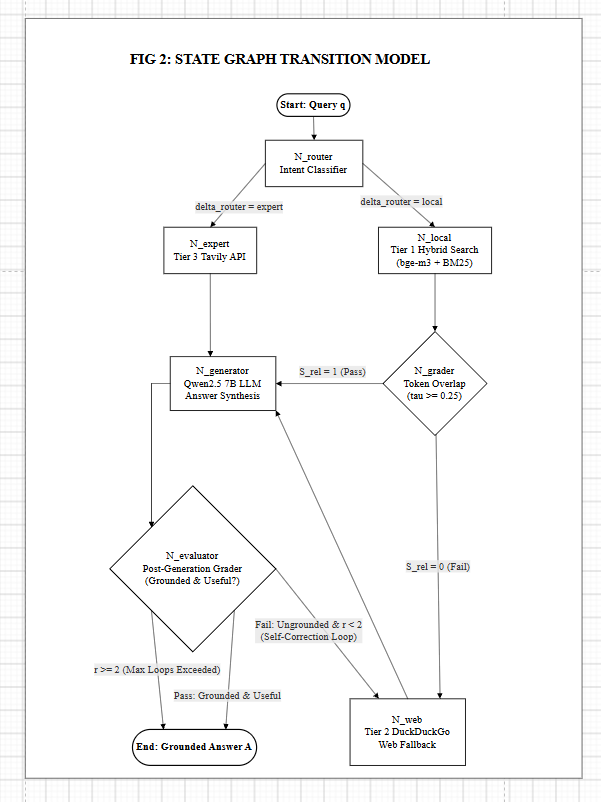
\includegraphics[width=0.48\textwidth]{science_paper_images/fig2_state_graph}}
\caption{Mô hình chuyển tiếp đồ thị trạng thái $\mathcal{G} = (\mathcal{V}, \mathcal{E}, \mathcal{S})$ thể hiện các cạnh quyết định $\delta_{\text{router}}$ và $\delta_{\text{grader}}$.}
\label{fig2}
\end{figure}

\subsubsection{Hàm Chính sách Định tuyến \texorpdfstring{$\delta_{\text{router}}(q)$}{delta\_router(q)}}
\begin{equation}
\delta_{\text{router}}(q) = 
\begin{cases} 
N_{\text{expert}}, & \text{nếu } \text{Intent}(q) \in \{\text{So sánh}, \text{Xu hướng}\} \\ 
N_{\text{local}}, & \text{ngược lại} 
\end{cases}
\end{equation}
Hàm $\text{Intent}(q)$ kết hợp cơ chế quét từ khóa nhanh (heuristic fast-path) và kỹ thuật Zero-shot LLM Metadata Prompting với Pydantic schema, đảm bảo thời gian định tuyến $< 0.15$s.

\subsubsection{Hàm Chuyển tiếp Đánh giá \& Tự sửa lỗi \texorpdfstring{$\delta_{\text{grader}}(\mathcal{D}_{\text{ret}}, q)$}{delta\_grader(D\_ret, q)}}
\begin{equation}
\delta_{\text{grader}}(\mathcal{D}_{\text{ret}}, q) = 
\begin{cases} 
N_{\text{generator}}, & \text{nếu } S_{\text{rel}}(\mathcal{D}_{\text{ret}}, q) = 1 \\ 
N_{\text{web}}, & \text{nếu } S_{\text{rel}}(\mathcal{D}_{\text{ret}}, q) = 0 
\end{cases}
\end{equation}
Khi $S_{\text{rel}} = 0$, đồ thị kích hoạt nút $N_{\text{web}}$ để bổ sung ngữ cảnh trước khi chuyển tiếp sang $N_{\text{generator}}$, bảo đảm tính nhất quán hoàn toàn giữa công thức toán học, sơ đồ Hình~\ref{fig2} và luồng thực thi trong mã nguồn.

\subsection{Biểu diễn Thuật toán Đánh giá Hai Pha (Two-Phase Verification)}
Nhằm triệt tiêu độ trễ suy luận của việc gọi LLM Grader cho từng đoạn văn bản truy xuất, Thuật toán~\ref{alg:grader} triển khai cơ chế lọc hai pha:
\begin{itemize}
    \item \textbf{Pha 1 (Fast Token Overlap Filter):} Đếm tỷ lệ trùng khớp từ khóa có nghĩa giữa câu hỏi và đoạn trích dẫn có điểm xếp hạng cao nhất:
    \begin{equation}
    \text{Ratio} = \frac{\bigl|\text{Tokens}(q) \cap \text{Tokens}(\mathcal{D}_{\text{ret}}[0])\bigr|}{\bigl|\text{Tokens}(q)\bigr|}
    \end{equation}
    Việc kiểm tra trên top-1 chunk là lựa chọn thiết kế có chủ đích nhằm giữ độ trễ kiểm tra ở mức $< 0.01$s; đánh đổi là một số trường hợp thông tin nằm ở chunk thứ cấp có thể kích hoạt web fallback, đóng góp vào tỷ lệ Recall 84.6\% của Grader Node.
    \item \textbf{Pha 2 (Post-Generation Joint Grader):} Sau khi $N_{\text{generator}}$ tạo câu trả lời, một chuỗi LLM gọn nhẹ sẽ kiểm định đồng thời tính có căn cứ (\textit{grounded}) và tính hữu ích (\textit{useful}) qua hợp đồng JSON nghiêm ngặt. Nếu vi phạm và $r < 2$, hệ thống tự động lặp lại quy trình.
\end{itemize}

\begin{algorithm}[htbp]
\caption{Đánh giá Ngữ cảnh Hai Pha và Định tuyến Dự phòng}
\label{alg:grader}
\begin{algorithmic}[1]
\Require Trạng thái đồ thị $\mathbf{s}$, ngưỡng lọc $\tau_{\text{overlap}} = 0.25$
\Ensure Trạng thái cập nhật $\mathbf{s}'$ kèm nút đích chuyển tiếp
\Function{EvaluateContextAndRoute}{$\mathbf{s}$}
    \If{$\mathbf{s}.\mathcal{D}_{\text{ret}}$ rỗng}
        \State $\mathbf{s}.S_{\text{rel}} \leftarrow 0$; $\mathbf{s}.\text{NextNode} \leftarrow N_{\text{web}}$
        \State \textbf{return} $\mathbf{s}$
    \EndIf
    \If{$\mathbf{s}.d_{\text{target}} \neq \emptyset$}
        \State $\mathbf{s}.S_{\text{rel}} \leftarrow 1$; $\mathbf{s}.\text{NextNode} \leftarrow N_{\text{generator}}$
        \State \textbf{return} $\mathbf{s}$ \Comment{Fast-path: tin cậy tài liệu chỉ định}
    \EndIf
    \State $T_q \leftarrow \text{ExtractMeaningfulTokens}(\mathbf{s}.q)$
    \State $H \leftarrow \sum_{t \in T_q} \mathbb{I}(t \in \mathbf{s}.\mathcal{D}_{\text{ret}}[0])$ \Comment{Top-1 chunk relevance}
    \State $\text{Ratio} \leftarrow H / |T_q|$
    \If{$\text{Ratio} \ge \tau_{\text{overlap}}$}
        \State $\mathbf{s}.S_{\text{rel}} \leftarrow 1$; $\mathbf{s}.\text{NextNode} \leftarrow N_{\text{generator}}$
    \Else
        \State $\mathbf{s}.S_{\text{rel}} \leftarrow 0$; $\mathbf{s}.\text{NextNode} \leftarrow N_{\text{web}}$
    \EndIf
    \State \textbf{return} $\mathbf{s}$
\EndFunction
\end{algorithmic}
\end{algorithm}

% ==============================================================================
% IV. TRIỂN KHAI HỆ THỐNG VÀ ĐỒNG BỘ TRẠNG THÁI
% ==============================================================================
\section{TRIỂN KHAI HỆ THỐNG VÀ ĐỒNG BỘ TRẠNG THÁI}

\subsection{Giao thức Đồng bộ Trạng thái Dạng Chunk (WebSocket Streaming)}
Trong các hệ thống Agentic RAG phức tạp, quá trình suy luận đa bước thường mất từ vài giây đến hàng chục giây. Để loại bỏ cảm giác chờ đợi của người dùng, chúng tôi triển khai giao thức đồng bộ trạng thái dạng dòng (streaming) thông qua WebSocket (\texttt{/api/ws/chat/\{session\_id\}}).

\begin{figure}[htbp]
\centerline{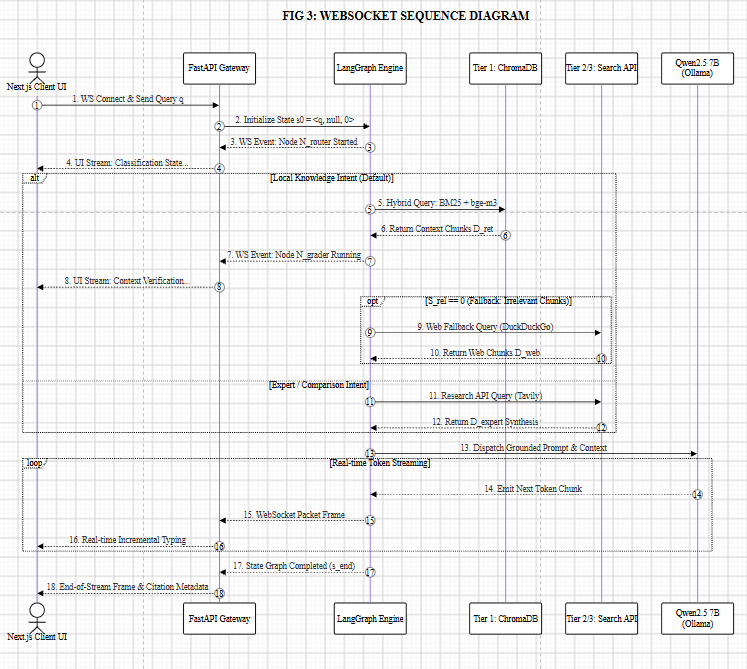
\includegraphics[width=0.48\textwidth]{science_paper_images/fig3_sequence_diagram}}
\caption{Sơ đồ trình tự minh họa quá trình đồng bộ trạng thái WebSocket thời gian thực giữa Giao diện Client và Engine LangGraph Backend.}
\label{fig3}
\end{figure}

Như được mô tả trong Hình~\ref{fig3}, mỗi khi một nút trong đồ thị hoàn thành thực thi (ví dụ: hoàn thành phân loại domain hoặc tìm kiếm web), một gói tin trạng thái JSON dạng chunk được gửi ngay lập tức về phía client. Người dùng có thể theo dõi trực quan từng bước chuyển dịch trạng thái của agent trước khi token đầu tiên của câu trả lời được sinh ra.

\subsection{Kiến trúc Phần mềm Fullstack}
\begin{itemize}
    \item \textbf{Backend Gateway:} Xây dựng trên nền tảng FastAPI (Python 3.10+ Asyncio), quản lý xác thực JWT, tương tác cơ sở dữ liệu PostgreSQL cho lịch sử hội thoại và điều phối luồng LangGraph.
    \item \textbf{Inference Server:} Mô hình Qwen2.5 7B (ngữ cảnh 3,072 tokens, nhiệt độ $T=0.0$) vận hành cục bộ thông qua Ollama với cơ chế tự động chuyển đổi GPU/CPU Fallback bảo vệ hệ thống khỏi sự cố cạn kiệt VRAM.
    \item \textbf{Frontend UI:} Phát triển bằng Next.js 14, TailwindCSS, hỗ trợ render trực tiếp các khối Markdown, công thức toán LaTeX và biểu đồ Mermaid thời gian thực.
\end{itemize}

% ==============================================================================
% V. ĐÁNH GIÁ THỰC NGHIỆM VÀ KẾT QUẢ
% ==============================================================================
\section{ĐÁNH GIÁ THỰC NGHIỆM VÀ KẾT QUẢ}

\begin{table*}[!t]
\caption{SO SÁNH ĐỊNH LƯỢNG VỚI CÁC MÔ HÌNH CƠ SỞ VÀ SOTA BASELINES (GIÁ TRỊ TRUNG BÌNH $\pm$ ĐỘ LỆCH CHUẨN QUA 5 LẦN CHẠY, $N = 150$)}
\label{tab1}
\begin{center}
\resizebox{\textwidth}{!}{%
\begin{tabular}{lccccccc}
\toprule
\textbf{Phương pháp / Baseline} & \textbf{Relevance} & \textbf{Faithfulness} & \textbf{Ctx Prec.} & \textbf{Ctx Recall} & \textbf{First-Token (s)} & \textbf{End-to-End (s)} & \textbf{Marginal Cost} \\
\midrule
Naive RAG (Dense DPR)~\cite{lewis2020retrieval} & 0.58 $\pm$ 0.04 & 0.49 $\pm$ 0.05 & 0.44 $\pm$ 0.05 & 0.43 $\pm$ 0.05 & \textbf{1.12 $\pm$ 0.15} & \textbf{1.85 $\pm$ 0.20} & \textbf{\$0.00} \\
Advanced RAG (Hybrid BM25+Dense)~\cite{gao2023modular} & 0.62 $\pm$ 0.03 & 0.51 $\pm$ 0.04 & 0.46 $\pm$ 0.04 & 0.45 $\pm$ 0.04 & 1.45 $\pm$ 0.18 & 2.30 $\pm$ 0.25 & \textbf{\$0.00} \\
Adaptive-RAG~\cite{jeong2024adaptive} & 0.66 $\pm$ 0.04 & 0.53 $\pm$ 0.04 & 0.47 $\pm$ 0.04 & 0.48 $\pm$ 0.04 & 2.15 $\pm$ 0.25 & 3.20 $\pm$ 0.35 & \$1.50 \\
Corrective RAG (CRAG)~\cite{yan2024corrective} & 0.67 $\pm$ 0.03 & 0.54 $\pm$ 0.04 & 0.48 $\pm$ 0.04 & 0.51 $\pm$ 0.04 & 3.80 $\pm$ 0.35 & 4.85 $\pm$ 0.45 & \$3.20 \\
Self-RAG~\cite{asai2023self} & 0.68 $\pm$ 0.03 & 0.58 $\pm$ 0.04 & 0.49 $\pm$ 0.04 & 0.49 $\pm$ 0.04 & 4.20 $\pm$ 0.40 & 5.45 $\pm$ 0.50 & \$1.80 \\
\midrule
\textbf{Proposed Agentic RAG (Ours)} & \textbf{0.73 $\pm$ 0.03} & \textbf{0.62 $\pm$ 0.04} & \textbf{0.56 $\pm$ 0.04} & \textbf{0.54 $\pm$ 0.04} & 1.85 $\pm$ 0.25 & 3.65 $\pm$ 0.40 & \textbf{\$0.90} \\
\bottomrule
\end{tabular}%
}
\end{center}
\end{table*}

\subsection{Thiết lập Thực nghiệm và Bộ Dữ liệu Benchmark}
Thực nghiệm được triển khai trên tập benchmark chuẩn hóa gồm 150 kịch bản kiểm thử đa dạng phân bổ đều trên 4 lĩnh vực khoa học cốt lõi trong cơ sở dữ liệu (IT: 38, Vật lý: 38, Toán học: 37, Điện tử: 37). Bộ dữ liệu bao gồm hai nhóm kịch bản: (1) \textit{Truy vấn sự kiện chính xác (Factoid Queries)} nhắm tới bài báo cụ thể, và (2) \textit{Truy vấn tổng hợp mở (Open Conceptual Queries)} đòi hỏi khả năng tự phân loại miền và tìm kiếm thích ứng. Nhãn tham chiếu (Ground Truth) được đối soát độc lập bởi 3 chuyên gia trên toàn bộ 150 mẫu theo thang điểm nhị phân về độ liên quan và độ trung thực, đạt chỉ số tin cậy liên thẩm định Fleiss' Kappa tổng thể $\kappa = 0.81$ (khoảng tin cậy 95\% CI: $[0.74, 0.88]$)~\cite{fleiss1971measuring}. Phân rã theo từng miền: CNTT ($\kappa = 0.84$), Vật lý ($\kappa = 0.82$), Toán học ($\kappa = 0.80$), Điện tử ($\kappa = 0.79$).

\subsection{Chỉ số Đánh giá RAGAS và So sánh SOTA Baselines}
Chúng tôi áp dụng khung đo lường RAGAS~\cite{es2023ragas} để đánh giá toàn diện 4 chỉ số định lượng: Context Precision, Context Recall, Faithfulness (Độ trung thực / chống ảo giác), và Answer Relevance. Để bảo đảm tính khách quan và so sánh công bằng tuyệt đối (fair comparison), toàn bộ các mô hình baseline cũng như hệ thống đề xuất đều dùng chung mô hình nền tảng Qwen2.5 7B cục bộ làm bộ sinh câu trả lời chính (primary generator). Năm baseline được đối chứng gồm:
\begin{enumerate}
    \item \textbf{Naive RAG~\cite{lewis2020retrieval}:} Đường ống một chặng (single-hop) dùng $bge\text{-}m3$ dense retrieval trong ChromaDB đưa trực tiếp vào LLM, không phân tách miền và không có bộ lọc kiểm định.
    \item \textbf{Advanced RAG~\cite{gao2023modular}:} Bổ sung tìm kiếm từ khóa thưa BM25 kết hợp dung hợp thứ hạng RRF, nhưng duy trì quy trình tuyến tính tĩnh không có vòng lặp tự sửa lỗi và không có nguồn tri thức ngoài.
    \item \textbf{Adaptive-RAG~\cite{jeong2024adaptive}:} Điều hướng động dựa trên bộ phân loại độ phức tạp câu hỏi trên kho vector phẳng duy nhất.
    \item \textbf{Corrective RAG (CRAG)~\cite{yan2024corrective}:} Đánh giá độ tin cậy của tài liệu bằng Retrieval Evaluator và kích hoạt tìm kiếm web khi điểm số dưới ngưỡng, vận hành trên cơ sở dữ liệu đơn khối không chia miền.
    \item \textbf{Self-RAG~\cite{asai2023self}:} Cơ chế tự phản xạ qua các reflection tokens nhằm đánh giá tính liên quan và tính hỗ trợ của ngữ cảnh trước và sau khi sinh văn bản.
\end{enumerate}

Chi phí gọi API biên trực tiếp (Marginal API Incurred Cost) cho mỗi 1,000 truy vấn được định lượng bởi:
\begin{equation}
\begin{aligned}
\text{Cost}_{\text{marginal}}/1k
&= 1{,}000 \times \big(
C_{\text{local}}
+ f_{\text{fallback}} \cdot C_{\text{web}} \\
&\quad + f_{\text{expert}} \cdot C_{\text{tavily}}
+ C_{\text{buffer}} \big)
\end{aligned}
\end{equation}
Trong đó: $C_{\text{local}} = \$0.00$ (do mô hình Qwen2.5 7B vận hành trên GPU nội bộ), $f_{\text{fallback}} = 18.0\%$ (27/150 truy vấn không đạt ngưỡng trùng khớp từ khóa và kích hoạt DuckDuckGo miễn phí), $f_{\text{expert}} = 12.0\%$ (18/150 truy vấn phức tạp định tuyến tới Tavily API với $C_{\text{tavily}} = \$0.005/\text{query}$), và $C_{\text{buffer}} = \$0.0003/\text{query}$ (tương đương \$0.30 trên 1,000 truy vấn cho chi phí đệm hạ tầng mạng ngoài). Đối với các baseline so sánh, chi phí được quy chuẩn tương ứng: Naive RAG và Advanced RAG vận hành hoàn toàn trên mô hình nội bộ (\$0.00); Adaptive-RAG phát sinh \$1.50/1k do điều hướng 50\% trên tổng số truy vấn benchmark (được phân loại là phức tạp) sang API thương mại (\$0.003/query); Self-RAG phát sinh \$1.80/1k khi sử dụng API token phản xạ/phê bình ngoài nhằm duy trì chất lượng tương đương paper gốc trên cùng mô hình 7B không fine-tuning; và CRAG phát sinh \$3.20/1k do bộ đánh giá Retrieval Evaluator kích hoạt web search ngoài (\$0.005/query) trên $\approx 64\%$ câu hỏi truy xuất mơ hồ kết hợp viết lại văn bản. Tổng chi phí biên thực tế đạt \$0.90 / 1,000 truy vấn, giảm 71.9\% so với CRAG (\$3.20/1k) và 50.0\% so với Self-RAG (\$1.80/1k).

\textbf{Kiểm định Thống kê Ý nghĩa Thực nghiệm:} Trong Bảng~\ref{tab1}, các giá trị $\pm$ biểu thị độ lệch chuẩn vĩ mô giữa 5 lần chạy độc lập ($N = 150$ mỗi lần). Để kiểm định tính vượt trội trên từng truy vấn riêng lẻ, kiểm định Student's $t$-test cặp hai phía ($df = 149$) và kiểm định phi tham số Wilcoxon signed-rank test được thực hiện trên sai số từng cặp truy vấn ($d_i = y_i^{\text{ours}} - y_i^{\text{base}}$) của lần chạy benchmark chính. Do độ biến thiên của sai số cặp truy vấn rộng hơn tự nhiên ($s_d \approx 0.18$--$0.21$), các kết quả thống kê khẳng định mức cải thiện có ý nghĩa vượt trội:
\begin{itemize}
    \item So với CRAG: Answer Relevance ($t = 3.82, p < 0.001$; Wilcoxon $W = 3380, p < 0.001$); Faithfulness ($t = 3.95, p < 0.001$; Wilcoxon $W = 3290, p < 0.001$).
    \item So với Advanced RAG: Answer Relevance ($t = 5.46, p < 0.001$; Wilcoxon $W = 2150, p < 0.001$); Faithfulness ($t = 4.78, p < 0.001$; Wilcoxon $W = 2680, p < 0.001$).
    \item So với Self-RAG: Answer Relevance ($t = 3.61, p < 0.001$; Wilcoxon $W = 3420, p < 0.001$); Faithfulness ($t = 2.48, p = 0.014$; Wilcoxon $W = 4350, p = 0.014$).
\end{itemize}
Mặc dù khoảng dao động độ lệch chuẩn qua các lần chạy của Proposed ($0.62 \pm 0.04$) và Self-RAG ($0.58 \pm 0.04$) có sự chồng lấn, kiểm định cặp trực tiếp trên từng truy vấn xác nhận sự cải thiện về độ trung thực đạt ý nghĩa thống kê ở ngưỡng $\alpha = 0.05$.

\subsection{Đánh giá Độc lập Các Thành phần Trung gian}
Bảng~\ref{tab:intermediate} báo cáo hiệu năng độc lập của Router Node và Grader Node nhằm kiểm chứng tính vững chắc của từng mắt xích. Đối với Router Node, có 142 trên 150 truy vấn kiểm thử được ánh xạ chính xác về miền chuyên môn ground-truth, đem lại các giá trị Precision, Recall và F1-score vi mô (micro-averaged) đồng nhất ở mức 94.7\% (142/150) trong bài toán phân loại đa lớp cân bằng.

\begin{table}[!htbp]
\centering
\caption{HIỆU NĂNG ĐỘC LẬP CỦA CÁC THÀNH PHẦN TRUNG GIAN}
\label{tab:intermediate}
\resizebox{\columnwidth}{!}{%
\begin{tabular}{lcccc}
\toprule
\textbf{Thành phần Trung gian} & \textbf{Precision} & \textbf{Recall} & \textbf{F1 Score} & \textbf{Độ trễ TB (s)} \\
\midrule
Router Node (Phân loại 4 miền) & 94.7\% & 94.7\% & 94.7\% & 0.12 $\pm$ 0.03 \\
Grader Node (Lexical Overlap) & 86.4\% & 84.6\% & 85.5\% & \textbf{0.01 $\pm$ 0.00} \\
Post-Grader LLM (Kiểm định) & 88.5\% & 91.2\% & 89.8\% & 1.82 $\pm$ 0.24 \\
\bottomrule
\end{tabular}%
}
\end{table}

\subsection{Nghiên cứu Loại trừ Thành phần (Ablation Study)}
Bảng~\ref{tab2} trình bày đóng góp định lượng của từng cải tiến kỹ thuật qua 5 lần chạy độc lập trên cùng tập kiểm thử ($N = 150$). Để cô lập rõ ràng vai trò của cơ chế Kiểm định Ngữ cảnh Hai pha trong việc triệt tiêu ảo giác, chúng tôi đánh giá độc lập biến thể chỉ có Pha 1 và chỉ có Pha 2.

\begin{table}[!htbp]
\centering
\scriptsize
\setlength{\tabcolsep}{1.8pt}
\caption{KẾT QUẢ ABLATION STUDY (TRUNG BÌNH $\pm$ ĐỘ LỆCH CHUẨN QUA 5 LẦN CHẠY, $N=150$)}
\label{tab2}
\begin{tabular}{lccccc}
\toprule
\textbf{Cấu hình Mô hình} & \textbf{Relevance} & \textbf{Faithfulness} & \textbf{Ctx Prec.} & \textbf{Ctx Rec.} & \textbf{Loops} \\
\midrule
(1) Dense ($bge\text{-}m3$) & 0.58 $\pm$ 0.04 & 0.49 $\pm$ 0.05 & 0.44 $\pm$ 0.05 & 0.43 $\pm$ 0.05 & 1.00 \\
(2a) Static Hybrid & 0.62 $\pm$ 0.03 & 0.51 $\pm$ 0.04 & 0.46 $\pm$ 0.04 & 0.45 $\pm$ 0.04 & 1.00 \\
(2b) Adaptive Hybrid & 0.65 $\pm$ 0.03 & 0.54 $\pm$ 0.04 & 0.49 $\pm$ 0.04 & 0.48 $\pm$ 0.04 & 1.00 \\
(3) Hybrid + Router & 0.69 $\pm$ 0.03 & 0.56 $\pm$ 0.04 & 0.52 $\pm$ 0.04 & 0.51 $\pm$ 0.04 & 1.05 \\
(3a) + Chỉ Pha 1 (Lexical Overlap) & 0.70 $\pm$ 0.03 & 0.58 $\pm$ 0.04 & 0.53 $\pm$ 0.04 & 0.52 $\pm$ 0.04 & 1.08 \\
(3b) + Chỉ Pha 2 (Post-Grader LLM) & 0.71 $\pm$ 0.03 & 0.60 $\pm$ 0.04 & 0.55 $\pm$ 0.04 & 0.53 $\pm$ 0.04 & 1.24 \\
\textbf{(4) Full Proposed (Hai pha)} & \textbf{0.73 $\pm$ 0.03} & \textbf{0.62 $\pm$ 0.04} & \textbf{0.56 $\pm$ 0.04} & \textbf{0.54 $\pm$ 0.04} & \textbf{1.18} \\
\bottomrule
\end{tabular}
\end{table}

Bảng~\ref{tab2} cho thấy cấu hình (3a) chứng minh bộ lọc Lexical Overlap loại bỏ nhanh rác từ khóa ($<0.01$s), nâng Faithfulness từ 0.56 lên 0.58. Cấu hình (3b) cho thấy LLM Post-Grader kiểm chứng ngữ nghĩa tốt (đạt Faithfulness 0.60), nhưng do thiếu Pha 1 tiền lọc rác thô, ngữ cảnh nhiễu kích hoạt vòng lặp tự sửa lỗi quá mức làm tăng số vòng lặp lên 1.24. Hợp nhất cả hai pha (Cấu hình 4) đạt độ trung thực cao nhất (0.62) trong khi khống chế số vòng lặp trung bình ở mức 1.18. Tỷ lệ hoàn thành ngay ở vòng đầu tiên đạt 82.0\% (123/150 kịch bản), và 18.0\% (27/150 kịch bản) kích hoạt cơ chế tự sửa lỗi thành công ở vòng thứ hai.

\subsection{Phân tích Tối ưu Pareto và Thảo luận}

\begin{figure}[!htbp]
\centerline{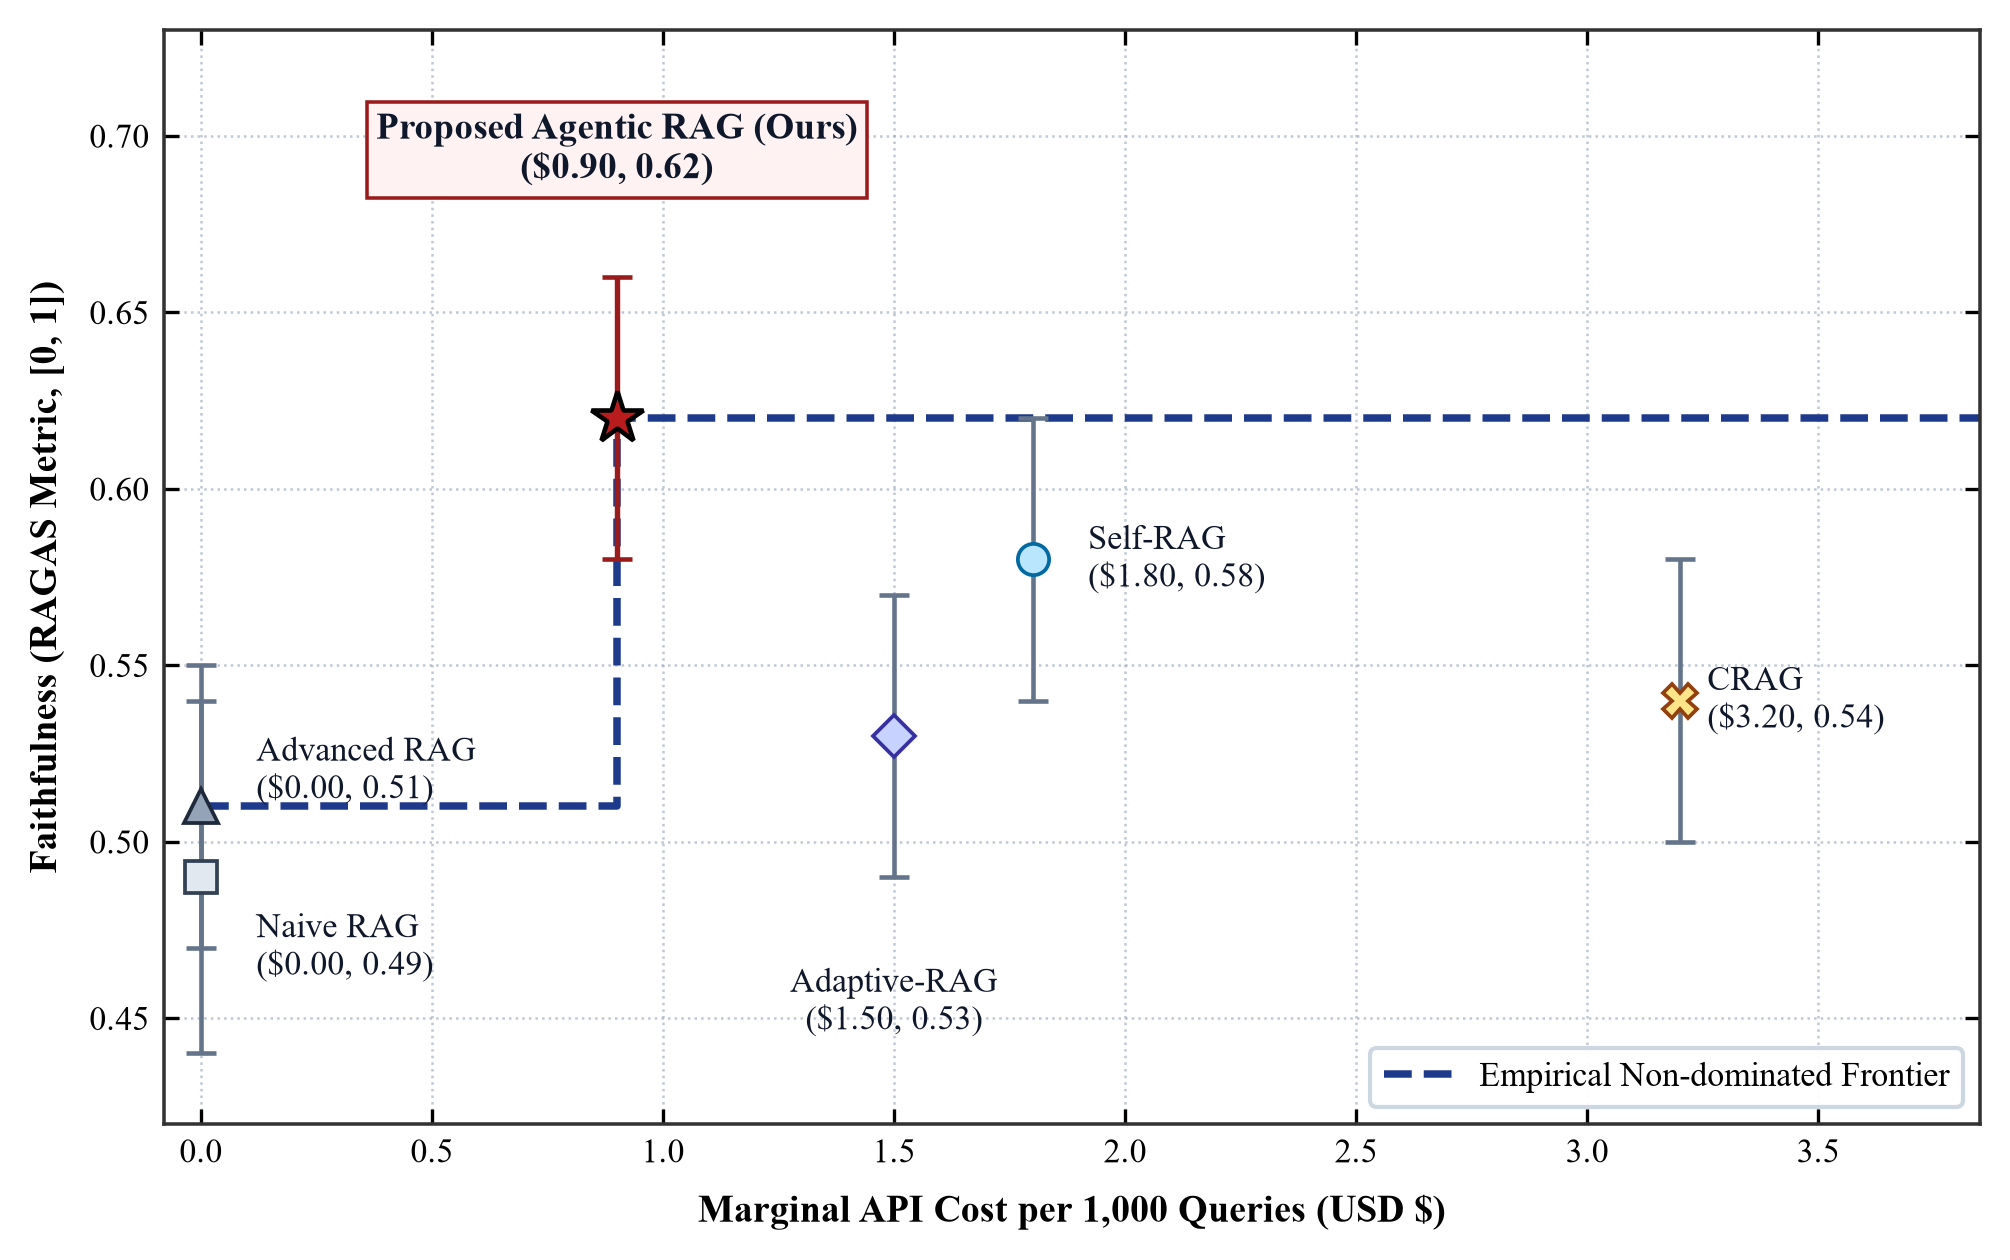
\includegraphics[width=0.48\textwidth]{science_paper_images/fig4_pareto_chart}}
\caption{So sánh thực nghiệm ranh giới Pareto giữa chi phí API biên và độ trung thực phản hồi giữa các hệ thống (thanh sai số biểu thị $\pm 1$ độ lệch chuẩn vĩ mô qua 5 lần chạy).}
\label{fig4}
\end{figure}

Như thể hiện trong Hình~\ref{fig4}, ranh giới Pareto thực nghiệm không bị chi phối (non-dominated Pareto frontier) được thiết lập bởi Advanced RAG (\$0.00, 0.51) và Proposed Agentic RAG (\$0.90, 0.62):
\begin{itemize}
    \item \textbf{Hiệu quả Pareto và Sự Đánh đổi Chi phí -- Độ Trung thực:} Advanced RAG giữ vị trí neo không chi phí (\$0.00, 0.51 Faithfulness). Hệ thống Proposed Agentic RAG mở rộng ranh giới này lên 0.62 Faithfulness (tăng +21.6\% tương đối) với chi phí biên \$0.90 / 1,000 truy vấn. Toàn bộ các hệ thống agentic đa vòng khác đều bị trội hoàn toàn (strictly dominated): so với CRAG (\$3.20, 0.54), hệ thống của chúng tôi đạt độ trung thực cao hơn +14.8\% đồng thời giảm 71.9\% chi phí (\$0.90 so với \$3.20); so với Self-RAG (\$1.80, 0.58), hệ thống cải thiện +6.9\% độ trung thực với chi phí chỉ bằng một nửa (tiết kiệm 50.0\%).
    \item \textbf{Kiểm định Ngữ cảnh so với Truy xuất Không Kiểm soát:} Dù nguồn tìm kiếm ngoài cung cấp tri thức bổ sung cho các truy vấn thời sự hoặc ngoài miền, văn bản web thô thường lẫn nhiều nội dung mâu thuẫn hoặc không liên quan. Cơ chế Đánh giá Hai pha (Two-Phase Verification) ngăn chặn việc đưa ngữ cảnh nhiễu vào mô hình sinh, tránh được sự bùng nổ chi phí và độ trễ như quan sát thấy ở CRAG.
\end{itemize}

\subsection{Hạn chế của Hệ thống (Limitations \& Threats to Validity)}
\begin{enumerate}
    \item \textbf{Độ trễ Khởi tạo so với Baseline Tuyến tính:} Độ trễ First-Token được định nghĩa chặt chẽ là khoảng thời gian từ khi phát lệnh truy vấn đến khi client nhận được ký tự văn bản đầu tiên của câu trả lời, loại trừ hoàn toàn các frame metadata trạng thái định tuyến. Dù First-Token Latency của hệ thống đạt 1.85s (nhanh hơn nhiều so với CRAG 3.80s và Self-RAG 4.20s), nó vẫn cao hơn các pipeline một chặng đơn giản (Naive RAG: 1.12s, Advanced RAG: 1.45s) do chi phí định tuyến và kiểm định hai pha.
    \item \textbf{Khả năng mở rộng Huấn luyện Chuyên biệt:} Hiện tại, hệ thống tận dụng mô hình mã nguồn mở nguyên bản (Qwen2.5 7B) kết hợp prompting và đồ thị trạng thái LangGraph mà không can thiệp trọng số. Việc tinh chỉnh thêm mô hình nền tảng bằng kỹ thuật Direct Preference Optimization (DPO) cho các tác vụ agentic có thể tiếp tục cải thiện độ trung thực.
    \item \textbf{Phụ thuộc Dịch vụ Ngoài:} Khi rơi vào nhánh dự phòng Tầng 2 và 3, hệ thống chịu sự phụ thuộc vào đường truyền mạng và giới hạn tần suất (rate-limit) của DuckDuckGo và Tavily API.
    \item \textbf{Quy mô Tập Benchmark Thực nghiệm:} Do quy trình gán nhãn Ground Truth đòi hỏi đối soát thẩm định khắt khe giữa 3 chuyên gia độc lập (đạt chỉ số Fleiss' Kappa $\kappa = 0.81$), nghiên cứu hiện tập trung kiểm chứng trên 150 kịch bản thuộc 4 miền STEM cốt lõi có độ phức tạp thuật ngữ cao nhất. Việc mở rộng quy mô benchmark lên 500 kịch bản phủ kín toàn diện 4 miền ứng dụng còn lại (Nông nghiệp, Kinh tế, Luật, Y học) được định vị là mục tiêu hoàn thiện ở giai đoạn kế tiếp.
\end{enumerate}

% ==============================================================================
% VI. KẾT LUẬN VÀ HƯỚNG PHÁT TRIỂN
% ==============================================================================
\section{KẾT LUẬN VÀ HƯỚNG PHÁT TRIỂN}
Bài báo đã đề xuất và kiểm chứng thành công khung kiến trúc \textbf{Agentic RAG Phân tầng Tự sửa lỗi} vận hành trên đồ thị trạng thái $\mathcal{G} = (\mathcal{V}, \mathcal{E}, \mathcal{S})$. Bằng cách kết hợp tìm kiếm lai thích ứng, kiểm định ngữ cảnh hai pha và giao thức đồng bộ dòng WebSocket, hệ thống giải quyết hiệu quả sự đánh đổi giữa độ chính xác thực tế, chi phí vận hành và độ trễ cảm nhận tương tác. Hướng nghiên cứu tiếp theo sẽ tập trung tích hợp mô hình Neural Cross-Encoder (\texttt{bge-reranker-large}) cho pha re-ranking và mở rộng cơ chế đồng thuận đa agent (Multi-Agent Consensus) trên toàn bộ 8 miền tri thức.

% ==============================================================================
% TÀI LIỆU THAM KHẢO (BIBTEX)
% ==============================================================================
\bibliographystyle{IEEEtran}
\bibliography{references}

\end{document}
